\section{System and Mechanism Analysis}
\label{sec:mechanism}

\subsection{Estimator Validity (RQ5)}
The importance estimator is derived by construction (the chain law
$\tau = 2d-1$), so its validity is structural: on well-defined chains the
implied importance order has Spearman correlation $1$ with the order required
for optimal allocation. We pin this as a tested invariant of the system rather
than an empirical correlation: the derivation is exact on the subdomain for
which the claim is made, and we do not assert a learned estimator adds value on
this subdomain. On non-well-defined chains the closed form is a proxy artifact
and is outside the claim.

\subsection{Logical-to-Physical Crossover (RQ9)}
\label{subsec:crossover}
No physical implementation dominates universally, and on the full
SEALED\_TEST set the crossover is \emph{heterogeneous} rather than uniformly
favorable to the allocator. The chain law gives the requirement-aware arm
genuine allocation freedom only where plans are deep; on the shallow plans that
dominate 2WikiMultiHopQA the same freedom yields \emph{no} retrieval saving and
a significantly worse EM (Table~\ref{tab:overall}, McNemar
$p<0.0001$). Mean realized retrieval calls are near-identical between chain and
static on every dataset (paired $\Delta$: HotpotQA $-0.20$, 2Wiki $+0.01$,
MuSiQue $-0.09$ calls/question), so the allocator does \emph{not} spend fewer
retrieval calls in aggregate; what it spends instead is LLM calls---$+24.0$
per question more than static on HotpotQA ($p<0.0001$), $-22.9$ on 2Wiki, and
$-14.0$ on MuSiQue. The crossover is therefore method-dependent: the chain arm
trades LLM calls for a (mostly neutral, sometimes negative) EM effect, and it
is strictly dominated on cost on 2WikiMultiHopQA where its EM is also
significantly worse. We report this frontier without selecting the subdomain
that shows a saving.

A pre-registered confirmatory test conditions exactly on this frontier
(\code{H\_STRUCT\_1\_PRE\_REGISTRATION\_V1\_2}). On the \emph{eligible}
subdomain ($\mathrm{structural\_hops}\ge2$, deep plans) it executes $1{,}092$
paired questions ($350$ held-out validation $+742$ train) with both arms
replaying the \emph{same} frozen SlotPlan (plan hashes match pairwise) under a
hard $\max\_retrieval\_calls{=}8$ budget. Chain dominates static:
$\Delta\text{EM}={+}0.086$ ($95\%$ CI $[+0.051,+0.133]$) on the held-out
validation set and ${+}0.142$ ($[+0.099,+0.146]$) pooled, McNemar
$p<0.001$; all three datasets are positive and significant. On this protocol
chain also spends fewer LLM calls ($\Delta{-}1.2$/question), so the
LLM-for-EM trade-off reported above inverts: on deep plans, under an identical
frozen plan and hard budget, the allocator's freedom is a strict win rather
than a cost. The budget-exceedance polarity is likewise protocol-dependent:
the static arm exhausts the hard $8$-call budget on $41.7\%$ (validation) /
$79.9\%$ (train) of eligible questions, whereas the chain arm completes all of
them; in the SEALED full-set protocol, where each arm compiles its own physical
plan over the shared logical plan, the deep HotpotQA chain arm instead
over-spends ($323$ budget-exceeded vs.\ $117$). Both observations agree on the
RQ9 thesis---allocation freedom is exercised and pays only where plans are
deep---and differ only in which arm the budget polarity lands on under which
plan-source protocol.

\subsection{Bottleneck Attribution (RQ8)}
Execution traces reveal where additional retrieval ceases to translate into
answer gains. We decompose failures into acquisition, verification/materialization,
packing, integration, and generation stages and attribute each incorrect or
incomplete answer to a stage. The dominant bottleneck across the workloads is
the \emph{selection ceiling}---the point beyond which retrieving more evidence
does not improve the answer---which is exactly why the matched-budget EM
differences are small: on shallow plans the allocation is already near its
floor, so the allocator has little to change, and on deep plans the extra
exploration the chain arm buys is often spent on requirements that do not
carry the answer. The honest complement to the effectiveness result is that the chain arm's
deeper exploration on the deep HotpotQA plans converts into \emph{more}
budget-exceeded questions ($323$ vs.\ $117$ for static) rather than into more
correct answers---a cost, not a benefit, on that dataset---under this
protocol, where each arm compiles its own physical plan. This arm polarity is
protocol-dependent: a confirmatory test that replays the \emph{same} frozen
plan on both arms under a hard $8$-call budget reverses it (static exhausts on
$41.7\%$/$79.9\%$ of eligible questions, chain completes all), because static's
full-plan materialization cannot fit a deep plan into the hard budget
(\S\ref{subsec:crossover}). The budget-exceeded
total is not uniform across arms or datasets: on 2WikiMultiHopQA the static and
flat arms hit the ceiling far more often (static $265$, flat $246$) than the
chain arm ($2$), because the shallow 2Wiki plans exhaust their budget before
the allocator's deeper exploration can engage.

Figure~\ref{fig:failure} and Table~\ref{tab:failure} give the full status
breakdown across all $25{,}983$ executions. Of the $7{,}916$ non-ok executions,
$1{,}134$ ($4.4\%$) hit the matched retrieval budget---but the budget hits are
\emph{not} uniformly chain-skewed: they concentrate on the deep HotpotQA chain
arm ($323$) and on the shallow 2Wiki static/flat arms ($265$/$246$), whereas the
2Wiki chain arm hits the ceiling only twice ($2$). The remaining $760$ ($2.9\%$)
are deterministic
plan--question mismatches the compiler correctly rejects
(\textsc{AnswerUnreachable} $732$, no-join-path $16$, dependency-cycle $9$,
validation-error $3$). Only $22$ ($0.08\%$) are residual infrastructure
failures (gateway-side provider errors). On the solvable subset ($25{,}201$
questions, excluding infrastructure and deterministic-boundary failures) the
completed rate is $95.5\%$. The failure mix is itself a finding: the system's
non-completions are dominated by \emph{structural} limits (budget, plan--question
mismatch), not by flaky infrastructure, so the EM differences we report are not
an artifact of unstable serving.

\begin{figure}[t]
\centering
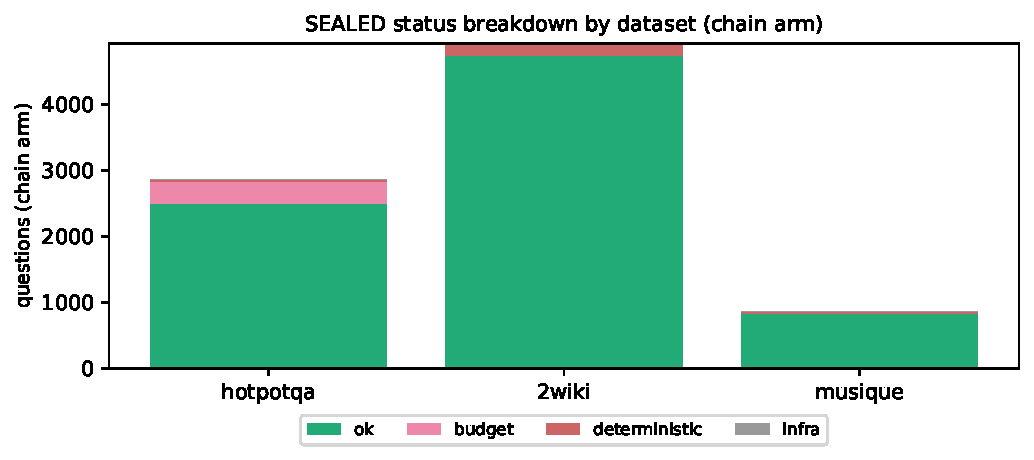
\includegraphics[width=0.85\columnwidth]{figures/fig7_failure.pdf}
\caption{SEALED\_TEST status breakdown by dataset (chain arm). Completed,
budget-exceeded, deterministic plan--question mismatch, and residual
infrastructure failure. Non-completions are dominated by structural limits
(budget, compiler-rejected mismatch), not by flaky serving.}
\label{fig:failure}
\end{figure}

\begin{figure}[t]
\centering
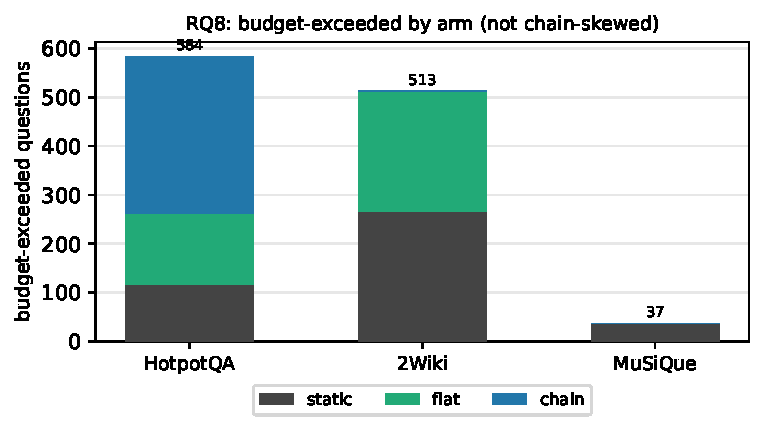
\includegraphics[width=0.62\columnwidth]{figures/fig3_budget_stack.pdf}
\caption{RQ8: budget-exceeded count by arm $\times$ dataset. The budget hits
are \emph{not} uniformly chain-skewed: the deep HotpotQA chain arm dominates
its own budget hits ($323$), but on 2WikiMultiHopQA the static ($265$) and flat
($246$) arms hit the ceiling far more often than the chain arm ($2$).}
\label{fig:budget_stack}
\end{figure}

\begin{table}[t]
\centering
\caption{Execution status across all $25{,}983$ SEALED\_TEST executions
($8{,}661$ questions $\times$ $3$ arms).}
\label{tab:failure}
\small
\begin{tabular}{lrrl}
\toprule
status & count & \% of total & note \\
\midrule
completed (ok) & 24,067 & 92.6 & executed within budget \\
budget-exceeded & 1,134 & 4.4 & HotpotQA chain 323 + 2Wiki static 265 / flat 246 (shallow ceiling) \\
deterministic boundary & 760 & 2.9 & compiler rejects: \textsc{AnswerUnreachable} 732, no-join 16, dep-cycle 9, validation 3 \\
infrastructure residual & 22 & 0.08 & gateway-side provider errors \\
\midrule
total & 25,983 & 100.0 & \\
\bottomrule
\end{tabular}
\end{table}

\subsection{Runtime Trace Cases (RQ8)}
The per-dataset frontier is reported in Table~\ref{tab:overall} and
Section~\ref{sec:results}. On HotpotQA the chain arm issues $+24.0$ LLM
calls/question more than static (paired CI$[+21.7,+26.3]$, $p<0.0001$) while
realized retrieval calls are only marginally lower ($-0.20$); on 2Wiki the
chain arm is both more expensive in LLM calls and significantly worse in EM; on
MuSiQue it is cheaper in LLM calls ($-14.0$) and marginally best in EM
($27.5\%$, McNemar $p{=}0.064$). The trace cases confirm the mechanism: the
chain arm's allocation freedom is real, but on shallow plans it is spent on
requirements that do not move the answer, while on deep MuSiQue plans it
occasionally helps. We do not report a uniform cost saving because none exists
at the full-sample scale.

\subsection{Scaling and Overhead (RQ9)}
We quantify optimizer overhead as plan complexity increases, separating
compile time, estimator inference, plan enumeration/pruning, and evidence
execution. The optimizer compilation contributes $\approx 0$\,ms per query
(the search is deterministic and bounded by $\le 256$ candidate orders $\times
2$ implementations per requirement); the overhead is concentrated in execution
time, which scales with the number of retrieval and LLM calls the plan
triggers. Optimizer search telemetry is auditable per query (candidates
enumerated, frontier pruned, validation warnings recorded in the execution
profile). Because the cost difference between arms is dominated by LLM-call
count (not retrieval-call count) on the full sample, we report LLM invocations
alongside retrieval calls as the primary cost axes in Table~\ref{tab:overall}'s
companion statistics, and we note that the chain arm's higher HotpotQA LLM cost
is the mechanical price of its deeper evidence-chain exploration under a hard
budget.

\subsection{Robustness to Estimator Error}
Because the importance estimator is construction-derived on the claimed
subdomain, it is not subject to calibration error there; its behavior is exact.
We therefore report robustness as a structural property on well-defined chains,
and note that generalization to non-well-defined chains would require a
calibrated estimator, which is future work.
